\begin{figure}[t]
\centering
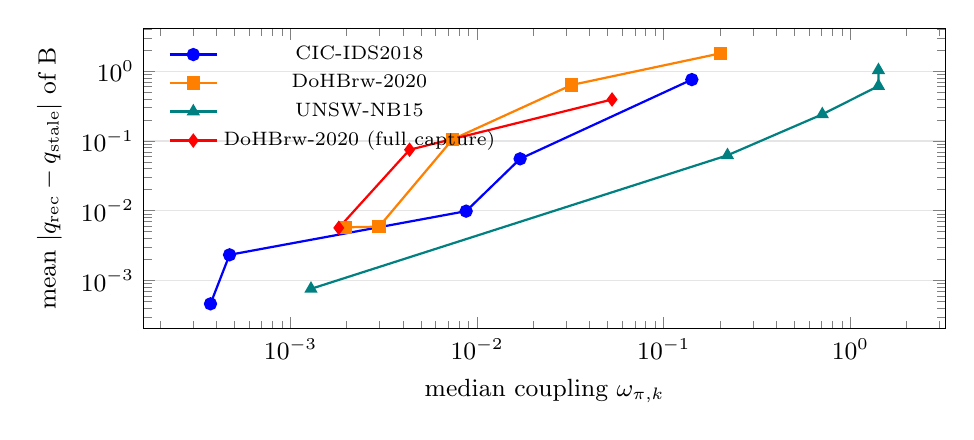
\begin{tikzpicture}
\begin{axis}[width=.97\linewidth,height=5.4cm,xmode=log,ymode=log,xlabel={median coupling $\omega_{\pi,k}$},ylabel={mean $|q_{\rm rec}-q_{\rm stale}|$ of B},tick label style={font=\small},label style={font=\small},ymajorgrids,grid style={black!10},legend style={at={(0.02,0.98)},anchor=north west,draw=none,font=\scriptsize,fill=none}]
\addplot[blue,thick,mark=*] coordinates {(0.0003725,0.0004625)(0.0004712,0.002334)(0.00873,0.00987)(0.01699,0.05555)(0.1414,0.7601)};
\addlegendentry{CIC-IDS2018}
\addplot[orange,thick,mark=square*] coordinates {(0.001961,0.005788)(0.00298,0.005909)(0.007385,0.1056)(0.03214,0.6368)(0.202,1.811)};
\addlegendentry{DoHBrw-2020}
\addplot[teal,thick,mark=triangle*] coordinates {(0.001287,0.0007587)(0.2195,0.06238)(0.7071,0.2412)(1.414,0.6139)(1.414,1.035)};
\addlegendentry{UNSW-NB15}
\addplot[red,thick,mark=diamond*] coordinates {(0.001814,0.005685)(0.004344,0.07497)(0.05284,0.394)};
\addlegendentry{DoHBrw-2020 (full capture)}
\end{axis}
\end{tikzpicture}
\caption{Stale-context score discrepancy grows with coupling on real alerts. Points, in order of decreasing window length: the full test snapshot (median coupling over the registered alerts), then wall-clock windows of $\Delta t\in\{600,60,10,1\}$\,s, each with a detector retrained on five seeds and 100 alerts per seed. The full-capture curve uses the complete DoHBrw-2020 layer-2 capture with $\Delta t\in\{60,10,1\}$\,s. On UNSW-NB15 the 10\,s and 1\,s windows share the median coupling $\sqrt2$ (both endpoints of degree one), so their points are stacked.}
\label{fig:coupling}
\end{figure}
